\clearpage
\section{Halmazok számossága}\label{sec-01-04}

\begin{definition}[Azonos számosságú halmazok]
  Ha két halmaz, $A$ és $B$ között kölcsönösen egyértelmű megfeleltetés hozható
  létre, akkor azt mondjuk, hogy a két halmaz számossága azonos. Jelölése:
  $\card A = \card B$.
\end{definition}

\begin{note}
  A számosság ekvivalenciareláció.
\end{note}

\begin{definition}[Véges halmaz]
  Az $A$ halmaz véges, ha $\exists n \in \mathbb N$, hogy $\card A = \card \; \{
    1; 2; \dots; n \}$, vagy ha $A = \emptyset$.
\end{definition}

\begin{note}
  Ha nincs olyan $n$ természetes szám, amelyre az $A \neq \emptyset$ halmaz
  ekvivalens volna az $\{ 1; 2; \dots; n \}$ halmazzal, akkor az $A$ halmazt
  végtelen számosságúnak mondjuk. Létezik megszámlálhatóan és
  megszámlálhatatlanul végtelen halmaz.
  \vspace{-5mm}
  \begin{center}
    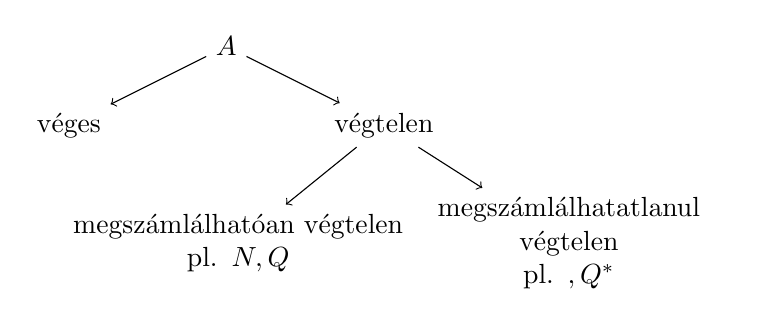
\begin{tikzpicture}
      % FIRST ROW
      \node (1) at (0,0) {$\card A$};

      % SECOND ROW
      \node (21) at (-2,-1) {véges};
      \node (22) at (2,-1) {végtelen};

      % CONNECT 1 -> 2
      \draw[->] (1) -- (21);
      \draw[->] (1) -- (22);

      % THIRD ROW
      \node[text width=4.5cm, align=center] (31) at (0.15,-2.5)
      {megszámlálhatóan végtelen\\pl. $\mathbb N, \mathbb Q$};
      \node[text width=4.5cm, align=center] (32) at (4.35,-2.5)
      {megszámlálhatatlanul végtelen\\pl. $\Reals, \mathbb Q^*$};

      % CONNECT 2 -> 3
      \draw[->] (22) -- (31);
      \draw[->] (22) -- (32);
    \end{tikzpicture}
  \end{center}
\end{note}

\begin{theorem}[Racionális számok halmazának számossága]
  A racionális számok halmaza megszámlálhatóan végtelen.

  \begin{proof}[Cantor átlós módszere]
    \begin{minipage}{.5\textwidth}
      Minden pozitív racionális szám felírható tört alakban, ahol a nevező és a
      számláló is egész szám, ráadásul ezek relatív prímek.
      \\[.33em]
      Ezeket a törteket rendezzük egy olyan táblázatba, ahol az $n$ sorban az
      $m$ oszlopban az $\sfrac{m}{n}$ tört áll. Ezeket a törteket az ábrán
      jelöl módszerrel sorba állítjuk, sorrendjük szerint pedig egyértelműen
      megfeleltethetők a természetes számoknak.
      \\[.33em]
      Könnyen belátható, hogy ez a módszer az összes racionális számra
      is kiterjeszthető, tehát a racionális számok halmaza valóban
      megszámlálhatóan végtelen.
      %\begin{noindent}
    \end{minipage}\hfill%
    \begin{minipage}{.425\textwidth}
      % \end{noindent}
      \begin{tikzpicture}[
          decoration={
              markings,
              mark=at position 0.5 with {\arrow{>}
                }
            }
        ]
        \draw[ultra thick, secondaryColor] (.5,-.5) rectangle (6.5,-7.5);

        \foreach \y in {1,...,6}{
            \foreach \x in {1,...,5}{
                \node (\x\y) at (\x,-\y) {$\sfrac{\x}{\y}$};
              }
          }

        \foreach \y in {1,...,6} {
            \node (6\y) at (6,-\y) {$\hdots$};
          }
        \foreach \x in {1,...,5}{
            \node (\x7) at (\x,-7) {$\vdots$};
          }
        \node(67) at (6,-7) {$\ddots$};

        \coordinate (P) at (11);
        \foreach \c in {12, 21, 31, 22, 13, 14, 23, 32, 41, 51, 42, 33, 24, 15, 16, 25, 34, 43, 52, 61}{
            \draw[postaction={decorate}, primaryColor, thick, opacity=0.5] (P) -- (\c.center);
            \coordinate (P) at (\c);
          }
      \end{tikzpicture}
    \end{minipage}
  \end{proof}
\end{theorem}

% \begin{theorem}[Valós számok halmazának számossága]
%   A valós számok halmaza nem megszámlálhatóan végtelen.
% \end{theorem}

% Ponthalmazok
\begin{blueBox}
  \sftitle{Fontosabb jelölések:}
  \begin{itemize}
    \item Nyílt halmaz jelölése: $(x; y) = ]x; y[$.
    \item Zárt halmaz jelölése: $[x; y]$.
    \item Az $a$ pont $\varepsilon$ sugarú környezete: $K(a; \varepsilon) := (a
          - \varepsilon; a + \varepsilon)$ \\ (ezzel ekvivalens: $|x-a| <
          \varepsilon$).
  \end{itemize}

  \begin{center}
    \begin{tikzpicture}
      % ARROW
      \draw[-to, ultra thick, secondaryColor] (-2,0) -- (2,0);

      % a point
      \draw[draw=primaryColor, ultra thick] (0,-1mm) -- ++(0,2mm)
      node[above] {$a$};

      % OPEN INTERVAL
      \draw[draw=primaryColor, ultra thick] (+10:1.25) arc (+10:-10:1.25)
      node[below] {$a + \varepsilon$};
      \draw[draw=primaryColor, ultra thick] (170:1.25) arc (170:190:1.25)
      node[below] {$a - \varepsilon$};
    \end{tikzpicture}
  \end{center}
\end{blueBox}

\begin{definition}[Alsó és felső korlát]
  A felülről korlátos $H$ halmaz legkisebb felső korlátja: supremum, jele: $\sup
    H$.
  \\
  Az alulról korlátos $H$ halmaz legnagyobb alsó korlátja: infimum, jele: $\inf
    H$.
\end{definition}

\begin{theorem}[Korlátos halmaz szuprémuma]
  Felülről korlátos nemüres halmaznak mindig van szuprémuma.
\end{theorem}

\begin{theorem}[Korlátos halmaz infimuma]
  Alulról korlátos nemüres halmaznak mindig van infimuma.
\end{theorem}